\documentclass[11pt]{article} % use larger type; default would be 10pt

\usepackage{pgfplots}
\usetikzlibrary{calc}
\usetikzlibrary{arrows}
\usetikzlibrary{patterns}
\usetikzlibrary{calc,intersections,through,backgrounds}
\usetikzlibrary{decorations.pathreplacing}
        \newcommand\degree[0]{^{\circ}}
        \newcommand\abs[1]{\left|#1\right|}

\title{Play with TikZ}
\author{Just Us}
%\date{} % Activate to display a given date or no date (if empty),
         % otherwise the current date is printed 

\begin{document}
\maketitle

\section{Chap 9 Vectors}

\subsection{9.3 The Dot Product}




fig9-3-1

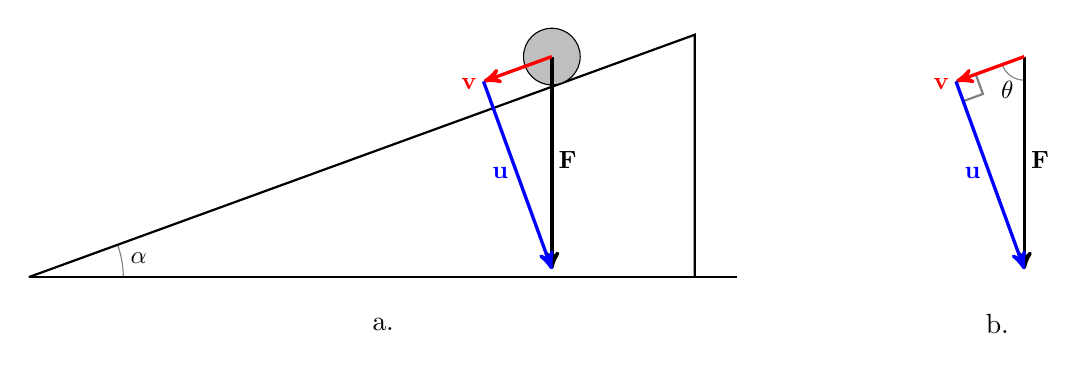
\begin{tikzpicture} [scale=.6]
\def\a{20};
\def\r{.6};
\def\w{4.5};
\coordinate (O) at ($ (\a:12) + ({\a +90}:\r) $);
\coordinate (F) at (-90:\w);

\draw[gray] (2,0) arc (0:\a:2) node[right, midway, yshift=1, text=black, scale=.9]{$\alpha$};
\draw[black, thick] (0,0)--++(15,0);
\draw[black,thick] (0,0)--++(\a:15)--($15*cos(\a)*(1,0)$);
\draw[black, fill=lightgray] (O) circle (\r);
\draw[black, very thick,->,>=stealth'] (O)--++(F) node[ right, midway, xshift=1,  yshift=1, scale=.9, fill=white, inner sep=1]{\textbf{F}};
\draw[red, very thick,->,>=stealth'] (O)--++($ \w*sin(\a)*({\a+180}:1)  $) node[ left, xshift=-1,  yshift=-1, scale=.9, fill=white, inner sep=1]{\textbf{v}};
\draw[blue, very thick,->,>=stealth'] ($ (O)+\w*sin(\a)*({\a+180}:1)  $)--++($ \w*cos(\a)*({\a-90}:1)  $) node[ left, midway, xshift=-2,  yshift=1, scale=.9, fill=white, inner sep=1]{\textbf{u}};
\node at (7.5,-1) {a.};

% second set
\coordinate (O) at ($ (10,0)+(\a:12) + ({\a +90}:\r) $);
\draw[gray] ($ (O) + (0,-.5)$) arc (-90:{\a-180}:.5) node[below left, midway, xshift=3, text=black, scale=.9, inner sep = 2]{$\theta$};


\draw[gray, thick] ($(O) + 3.2*sin(\a)*({\a+180}:1) $) --++ ($ 1.3*sin(\a)*({\a-90}:1) $)--++($ 1.3*sin(\a)*({\a+180}:1) $);
\draw[black, very thick,->,>=stealth'] (O)--++(F) node[ right, midway, xshift=1,  yshift=1, scale=.9, fill=white, inner sep=1]{\textbf{F}};
\draw[red, very thick,->,>=stealth'] (O)--++($ \w*sin(\a)*({\a+180}:1)  $) node[ left, xshift=-1,  yshift=-1, scale=.9, fill=white, inner sep=1]{\textbf{v}};
\draw[blue, very thick,->,>=stealth'] ($ (O)+\w*sin(\a)*({\a+180}:1)  $)--++($ \w*cos(\a)*({\a-90}:1)  $) node[ left, midway, xshift=-2,  yshift=1, scale=.9, fill=white, inner sep=1]{\textbf{u}};
\node at (20.5,-1) {b.};

\end{tikzpicture}
\newline


exam9-3-1

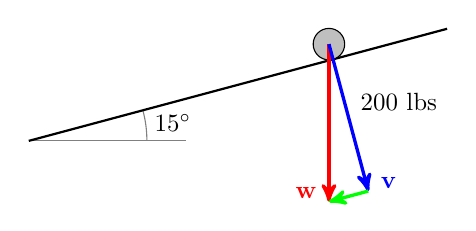
\begin{tikzpicture} [scale=1]
\def\a{15};
\def\r{.2};
\def\w{2};
\coordinate (O) at ($ (\a:4) + ({\a +90}:\r) $);
\coordinate (F) at (-90:\w);

\draw[gray] (1.5,0) arc (0:\a:1.5) node[right, midway, yshift=1, text=black, scale=.9]{$15 \degree$};
\draw[gray] (0,0)--++(2,0);
\draw[black,thick] (0,0)--++(\a:5.5);
\draw[black, fill=lightgray] (O) circle (\r);
\draw[red, very thick,->,>=stealth'] (O)--++(F) node[left, xshift=-3,  yshift=3, scale=.9, fill=white, inner sep=1]{\textbf{w}};
\draw[blue, very thick,->,>=stealth'] (O)--++($ \w*cos(\a)*({\a-90}:1)  $) node[right, xshift=1,  yshift=3, scale=.9]{\textbf{v}};
\draw[green, very thick,->,>=stealth'] ($ (O)+\w*cos(\a)*({\a-90}:1)  $)--++($ \w*sin(\a)*({\a+180}:1)  $);
\node[scale=.9] at (4.7,.5){200 lbs};
\end{tikzpicture}
\newline


exer9-3-1

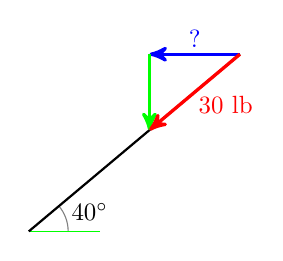
\begin{tikzpicture} [scale=0.05]
\coordinate (O) at (0,0);
\def\w{30};
\def\a{40};
\coordinate (F) at (220:\w);
\coordinate (A) at (\a:70);

\draw[gray] (10,0) arc (0:\a:10) node[right, midway, xshift=1, yshift=2, text=black, scale=.9, inner sep=1]{$40 \degree$};
\draw[green] (0,0)--++(18,0);
\draw[black,thick] (0,0)--++(A);
\draw[blue, very thick,->,>=stealth'] (A)--++($30*cos(\a)*(-1,0)$) node[above, yshift=1, midway,scale=.9,inner sep=1 ]{?};
\draw[green, very thick,->,>=stealth'] ($(A)+30*cos(\a)*(-1,0) $)--++($30*sin(\a)*(0,-1)$) ;
\draw[red, very thick,->,>=stealth'] (A)--++(F) node[below right, midway, scale=.9,inner sep=1 ]{30 lb};
\end{tikzpicture}
\newline


fig9-3-2

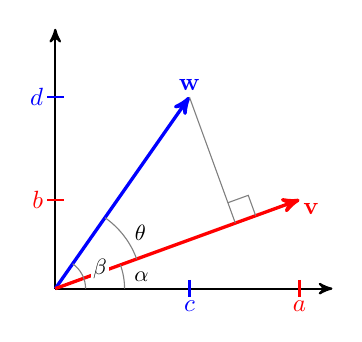
\begin{tikzpicture} [scale=1.1]
\coordinate (O) at (0,0);
\def\lv{3};
\def\lw{2.7};
\def\a{20};
\def\b{55};
\coordinate (v) at (\a:\lv);
\coordinate (vx) at ({\lv*cos(\a)},0);
\coordinate (vy) at (0,{\lv*sin(\a)});
\coordinate (w) at (\b:\lw);
\coordinate (wx) at ({\lw*cos(\b)},0);
\coordinate (wy) at (0,{\lw*sin(\b)});
\draw[black,thick,->,>=stealth'] (O)--(3.2,0);
\draw[black,thick,->,>=stealth'] (O)--(0,3);

\draw[blue, very thick,->,>=stealth'] (O)--++(w) node[above, yshift=1, scale=.9,inner sep=1 ]{\textbf{w}};
\draw[blue, thick] ($(wx)+(0,.1)$)--++(0,-.2) node[below, scale=.9,inner sep=1 ]{$c$};
\draw[blue, thick] ($(wy)+(.1,0)$)--++(-.2,0) node[left, scale=.9,inner sep=1 ]{$d$};
\draw[red, very thick,->,>=stealth'] (O)--++(v) node[below right, scale=.9,inner sep=1 ]{\textbf{v}};
\draw[red, thick] ($(vx)+(0,.1)$)--++(0,-.2) node[below, scale=.9,inner sep=1 ]{$a$};
\draw[red, thick] ($(vy)+(.1,0)$)--++(-.2,0) node[left, scale=.9,inner sep=1 ]{$b$};

\draw[gray] (0.35,0) arc(0:\b:0.35) node[right, midway, xshift=3, yshift=2, text=black, scale=.8, fill=white, inner sep=1]{$\beta$};
\draw[gray] (0.8,0) arc(0:\a:0.8) node[right, midway, xshift=3, text=black, scale=.8, fill=white, inner sep=1]{$\alpha$};
\draw[gray] (\a:1) arc(\a:\b:1) node[right, midway, xshift=3, yshift=1, text=black, scale=.8, fill=white, inner sep=1]{$\theta$};

\draw[gray] (w) -- ($ (w) + \lw*sin(\b-\a)*({\a-90}:1) $);
\draw[gray]  ($ (w) + \lw*sin(\b-\a)*({\a-90}:1)+({\a+90}:.25) $) --++(\a:.25)--++({\a-90}:.25);
\end{tikzpicture}
\newline


exam9-3-2

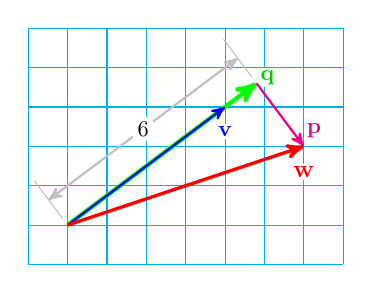
\begin{tikzpicture} [scale=.5]
\draw[cyan] (0,0) grid (8,6);
\coordinate (O) at (1,1);
\coordinate (v) at (4,3);
\coordinate (w) at (6,2);
\coordinate (q) at (24/5,18/5);
\coordinate (p) at (6/5, -8/5);

\draw[lightgray] ($(O)+(q)+-.1*(p)$)--++($-.6*(p)$);
\draw[lightgray] ($(O)+-.1*(p)$)--++($-.6*(p)$);
\draw[lightgray,  thick,<->,>=stealth'] ($(O)-.4*(p)$)--++(q) node[midway,  scale=.9,fill=white, inner sep=2, scale=.9, text=black]{6};
\draw[green, ultra thick,->,>=stealth'] (O)--++(q) node[above right , yshift=-2, scale=.9,fill=white, inner sep=1, scale=.9, text=green!80!black]{\textbf{q}};
\draw[magenta,  thick,->,>=stealth'] ($(O)+(q)$)--++(p) node[above right , yshift=2, scale=.9,fill=white, inner sep=1, scale=.9, text=magenta]{\textbf{p}};
\draw[blue, thick,->,>=stealth'] (O)--++(v) node[below , yshift=-6, scale=.9,fill=white, inner sep=1, scale=.9]{\textbf{v}};
\draw[red, very thick,->,>=stealth'] (O)--++(w) node[below, yshift=-6, scale=.9, fill=white,inner sep=1 ]{\textbf{w}};
\end{tikzpicture}
\newline


exam9-3-4.

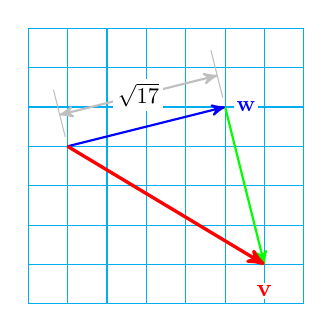
\begin{tikzpicture} [scale=.5]
\draw[cyan] (0,0) grid (7,7);
\coordinate (O) at (1,4);
\coordinate (v) at (5,-3);
\coordinate (w) at (4,1);
\coordinate (q) at ($ (v) - (w)$);

\draw[lightgray] ($(O)+-.06*(q)$)--++($-.3*(q)$);
\draw[lightgray] ($(O)+(w)+-.06*(q)$)--++($-.3*(q)$);
\draw[lightgray,  thick,<->,>=stealth'] ($(O)-.2*(q)$)--++(w) node[midway,  scale=.9,fill=white, inner sep=2, scale=.9, text=black]{$\sqrt{17}$};
\draw[green, thick,->,>=stealth'] ($(O)+(w)$)--++(q);
\draw[blue, thick,->,>=stealth'] (O)--++(w) node[right , xshift=3, scale=.9,fill=white, inner sep=1, scale=.9]{\textbf{w}};
\draw[red, very thick,->,>=stealth'] (O)--++(v) node[below, yshift=-6, scale=.9, fill=white,inner sep=1 ]{\textbf{v}};
\end{tikzpicture}
\newline



fig9-3-3 

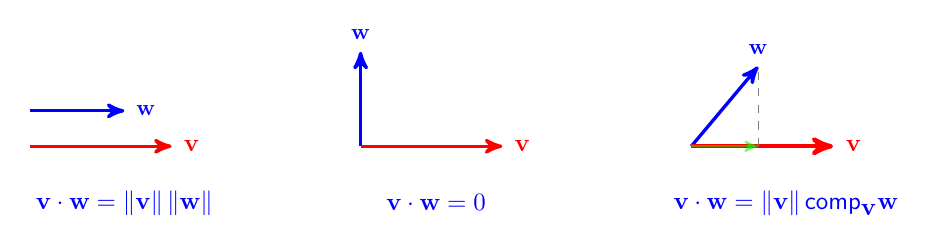
\begin{tikzpicture} [scale=.6]
\coordinate (O) at (0,0);
\coordinate (v) at (3,0);
\coordinate (w) at (2,0);

\draw[blue, very thick,->,>=stealth'] (0,.75)--++(w) node[right , xshift=3, scale=.9, inner sep=1, scale=.9]{\textbf{w}};
\draw[red, very thick,->,>=stealth'] (O)--++(v) node[right, xshift=3, scale=.9, inner sep=1 ]{\textbf{v}};
\node[text=blue, scale=.9] at (2,-1.2) {$ \textbf{v}\cdot\textbf{w}= \Vert\textbf{v}\Vert   \,  \Vert\textbf{w} \Vert  $};

\coordinate (O) at (7,0);
\coordinate (v) at (3,0);
\coordinate (w) at (0,2);

\draw[blue, very thick,->,>=stealth'] (O)--++(w) node[above, yshift=3, scale=.9, inner sep=1, scale=.9]{\textbf{w}};
\draw[red, very thick,->,>=stealth'] (O)--++(v) node[right, xshift=3, scale=.9, inner sep=1 ]{\textbf{v}};
\node[text=blue, scale=.9] at ($(O)+(1.6,-1.2)$) {$ \textbf{v}\cdot\textbf{w}= 0 $};

\coordinate (O) at (14,0);
\coordinate (v) at (3,0);
\def\a{50};
\def\r{2.2}
\coordinate (w) at (\a:\r);
\coordinate (c) at ( {\r*cos(\a)},0);

\draw[blue, very thick,->,>=stealth'] (O)--++(w) node[above, yshift=3, scale=.9, inner sep=1, scale=.9]{\textbf{w}};
\draw[red, ultra thick,->,>=stealth'] (O)--++(v) node[right, xshift=3, scale=.9, inner sep=1 ]{\textbf{v}};
\draw[green, thick,->,>=stealth', opacity = .5] (O)--++(c);
\draw[gray, dashed] ($ (O)+(c)$) --($ (O) + (w) $);
\node[text=blue, scale=.9] at ($(O)+(2,-1.2)$) {$ \textbf{v}\cdot\textbf{w}= \Vert\textbf{v}\Vert \,\textsf{comp}_{\textbf{v}} \textbf{w} $};
\end{tikzpicture}
\newline



fig9-3-3 

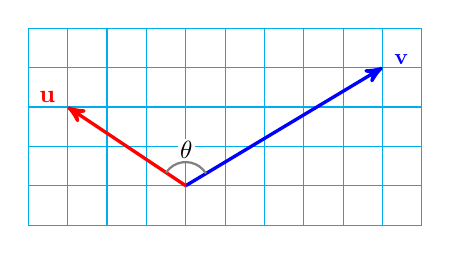
\begin{tikzpicture} [scale=.5]
\draw[cyan] (0,0) grid (10,5);
\coordinate (O) at (4,1);
\coordinate (v) at (5,3);
\coordinate (u) at (-3,2);

\draw[blue, very thick,->,>=stealth'] (O)--++(v) node[above right , xshift=3, scale=.9, inner sep=1, scale=.9]{\textbf{v}};
\draw[red, very thick,->,>=stealth'] (O)--++(u) node[above left, xshift=-3, scale=.9, inner sep=1 ]{\textbf{u}};
\draw[gray,thick] ($ (O) + ({atan(3/5)}:.6) $) arc({atan(3/5)}:{180-atan(2/3)}:.6) node[above, midway, text=black, fill=white, inner sep=1, scale=.9]{$\theta$}; 
\end{tikzpicture}
\newline



sr9-3-1

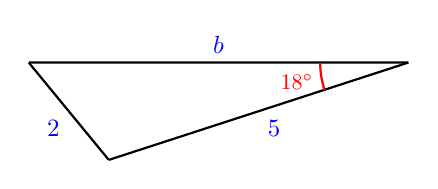
\begin{tikzpicture} [scale=.8]
\coordinate (C) at (0,0);
\coordinate (A) at (198:5);
\def\beta{asin(sin(18)/2*5)};
\def\alpha{180-18-\beta};
\coordinate (B) at ($ (A) + ({180-\beta}:2)  $);

\draw[black,  thick] (C)--(A) node[below right, midway, scale=.9, text=blue]{5};
\draw[black,  thick] (B)--(A) node[below left, midway, scale=.9, text=blue]{2};
\draw[black,  thick] (C)--(B) node[above, midway,  scale=.9, text=blue]{$b$};
\draw[red,  thick] (-1.4,0) arc(180:198:1.4) node[left, midway, yshift=-2,  scale=.8]{$18\degree$};
\end{tikzpicture}
\newline



sr9-3-2

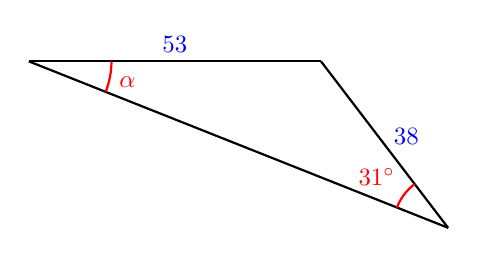
\begin{tikzpicture} [scale=.07]
\coordinate (C) at (0,0);
\coordinate (B) at (53,0);
\def\c{31};
\def\a{asin(sin(\c)/53*38)};
\def\b{180-\c-\a};
\coordinate (A) at ($ (B) + ({\b-180}:38)  $);

\draw[black,  thick] (C)--(A) ;
\draw[black,  thick] (B)--(A) node[right, midway, yshift=3, scale=.9, text=blue]{38};
\draw[black,  thick] (C)--(B) node[above, midway, scale=.9, text=blue]{53};
\draw[red,  thick] (15,0) arc(0:-\a:15) node[right, midway, yshift=-2, scale=.9]{$\alpha$};
\draw[red,  thick] ($ (A)+({\b}:10) $) arc({\b}:{\b+\c}:10) node[above left, midway, scale=.9]{$31\degree$};
\end{tikzpicture}
\newline



sr9-3-3

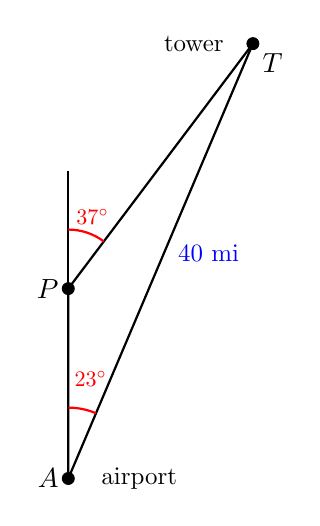
\begin{tikzpicture} [scale=.15]
\coordinate (A) at (0,0);
\def\a{23};
\coordinate (T) at ({90-\a}:40);
\def\x{40*sin(\a};
\def\b{37};
\coordinate (P) at ($ (T) + ({270-\b}:{40*sin(\a)/sin(\b)}) $);

\draw[black,  thick] (A)--(T) node[right, midway, xshift=3, yshift=3, scale=.9, text=blue]{40 mi} ;
\draw[black,  thick] (A)--(P)--(T);
\draw[black,  thick] (P)--++(90:10);
\draw[red,  thick] (0,6) arc(90:{90-\a}:6) node[above, midway, xshift=3, yshift=5, scale=.8]{$\a\degree$};
\draw[red,  thick] ($ (P)+(90:5) $) arc(90:{90-\b}:5) node[above, midway, xshift=2, scale=.8]{$\b\degree$};
\filldraw[black] (A) circle (.5) node[left]{$A$};
\filldraw[black] (P) circle (.5) node[left]{$P$};
\filldraw[black] (T) circle (.5) node[below right]{$T$};
\node[scale=.9] at (6,0) {airport};
\node[scale=.9] at ($ (T)+(-5,0) $) {tower};
\end{tikzpicture}
\newline



sr9-3-4

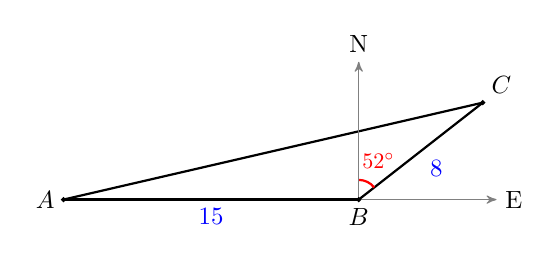
\begin{tikzpicture} [scale=.25]
\coordinate (A) at (-15,0);
\coordinate (B) at (0,0);
\coordinate (C) at (38:8);

\draw[black,  thick] (A)--(B) node[below, midway, scale=.9, text=blue]{15};
\draw[black,  thick] (A)--(C);
\draw[black,  thick] (B)--(C)node[below right, midway, scale=.9, text=blue]{8};
\draw[red,  thick] (0,1) arc(90:38:1) node[above, midway, xshift=4, yshift=2, scale=.8]{$52\degree$};
\draw[gray, ->, >=stealth'] (B) -- (0,7) node[above, scale=.9, text=black]{N};
\draw[gray, ->, >=stealth'] (B) -- (7,0) node[right, scale=.9, text=black]{E};
\filldraw[black] (A) circle (.1) node[left, scale=.9]{$A$};
\filldraw[black] (B) circle (.1) node[below, scale=.9]{$B$};
\filldraw[black] (C) circle (.1) node[above right, scale=.9]{$C$};
\end{tikzpicture}
\newline


hmwk 1.3.25b called this eight-grid with easy arrow-heads, more tick marks

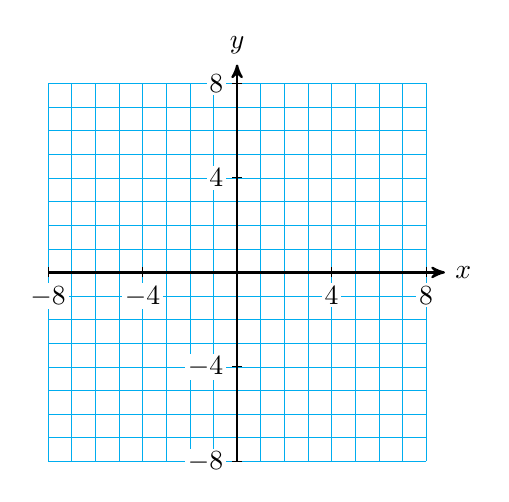
\begin{tikzpicture} [scale =0.3]

\draw[step=1cm,cyan,very thin] (-8,-8) grid (8,8);
\draw[thick,->, >=stealth'] (-8,0) -- (8.8,0) node[anchor=west] {$x$};
\draw[thick,->, >=stealth'] (0,-8) -- (0,8.8) node[anchor=south] {$y$};
`
\foreach \x in {-8,-4,4,8}
    \draw (\x cm,6pt) -- (\x cm,-6pt) node[anchor=north, fill=white, inner sep=1, yshift=-2] {$\x$};
\foreach \y in {-8,-4,4,8}
    \draw (6pt,\y cm) -- (-6pt,\y cm) node[anchor=east, fill=white, inner sep=1, xshift=-2] {$\y$};

\end{tikzpicture}
\newline


hp9-3-7ans

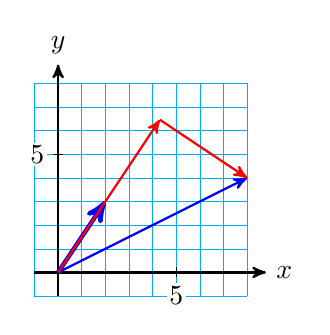
\begin{tikzpicture} [scale =0.3]

\draw[cyan,very thin] (-1,-1) grid (8,8);
\draw[thick,->, >=stealth'] (-1,0) -- (8.8,0) node[anchor=west] {$x$};
\draw[thick,->, >=stealth'] (0,-1) -- (0,8.8) node[anchor=south] {$y$};

\coordinate (O) at (0,0);
\coordinate (w) at (8,4);
\coordinate (v) at (2,3);
\coordinate (wv) at ($ 28/13*(v)$);
\coordinate (wp) at ($ (w) - (wv)  $);

\foreach \x in {5} {
    \draw (\x cm,6pt) -- (\x cm,-6pt) node[anchor=north, fill=white, inner sep=1, yshift=-2] {$\x$};
    \draw (6pt,\x cm) -- (-6pt,\x cm) node[anchor=east, fill=white, inner sep=1, xshift=-2] {$\x$};}

\draw[blue, ultra thick, ->,>=stealth'] (O) --(v);
\draw[blue, thick, ->,>=stealth'] (O) --(w);
\draw[red, thick, ->,>=stealth'] (O) --(wv);
\draw[red, thick, ->,>=stealth'] (wv) --++(wp);

\end{tikzpicture}
\newline


hp9-3-9ans

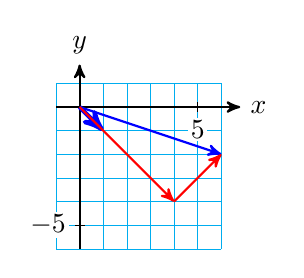
\begin{tikzpicture} [scale =0.3]

\draw[cyan,very thin] (-1,-6) grid (6,1);
\draw[thick,->, >=stealth'] (-1,0) -- (6.8,0) node[anchor=west] {$x$};
\draw[thick,->, >=stealth'] (0,-6) -- (0,1.8) node[anchor=south] {$y$};

\coordinate (O) at (0,0);
\coordinate (w) at (6,-2);
\coordinate (v) at (1,-1);
\coordinate (wv) at ($ 4*(v)$);
\coordinate (wp) at ($ (w) - (wv)  $);

\foreach \x in {5} {
    \draw (\x cm,6pt) -- (\x cm,-6pt) node[anchor=north, fill=white, inner sep=1, yshift=-2] {$\x$};
    \draw (6pt,-\x cm) -- (-6pt,-\x cm) node[anchor=east, fill=white, inner sep=1, xshift=-2] {$-\x$};}

\draw[blue, ultra thick, ->,>=stealth'] (O) --(v);
\draw[blue, thick, ->,>=stealth'] (O) --(w);
\draw[red, thick, ->,>=stealth'] (O) --(wv);
\draw[red, thick, ->,>=stealth'] (wv) --++(wp);

\end{tikzpicture}
\newline


hp9-3-17

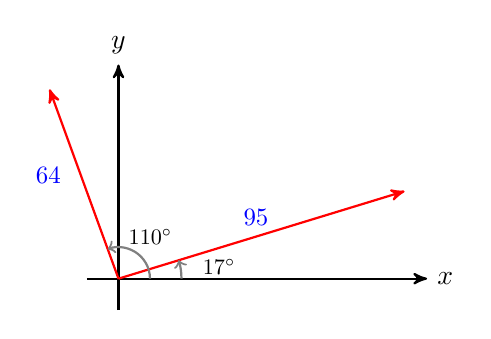
\begin{tikzpicture} [scale =0.04]

\draw[thick,->, >=stealth'] (-10,0) -- (98,0) node[anchor=west] {$x$};
\draw[thick,->, >=stealth'] (0,-10) -- (0,68) node[anchor=south] {$y$};

\coordinate (O) at (0,0);
\coordinate (w) at (17:95);
\coordinate (v) at (110:64);

\draw[red, thick, ->,>=stealth'] (O) --(v) node[left, midway, xshift=-5, yshift=3, scale=.9, text=blue]{64};
\draw[red, thick, ->,>=stealth'] (O) --++(w) node[above, midway, xshift=-2, scale=.9, text=blue]{95};
v
\draw[gray,thick,->] (0:20) arc (0:17:20) node[right, xshift=5, yshift=1, midway, text=black, scale=.8]{$17\degree$};
\draw[gray,thick,->] (0:10) arc (0:110:10) node[above, xshift=5, midway, text=black, scale=.8]{$110\degree$};

\end{tikzpicture}
\newline


hp9-3-18

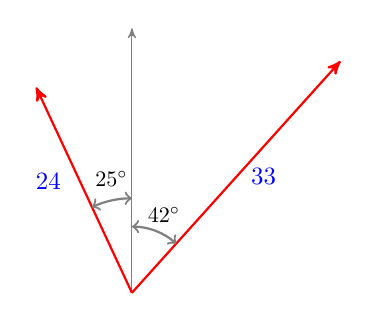
\begin{tikzpicture} [scale =0.12]

\draw[gray,->, >=stealth'] (0,0) -- (0,28);

\coordinate (O) at (0,0);
\coordinate (w) at (115:24);
\coordinate (v) at (48:33);

\draw[red, thick, ->,>=stealth'] (O) --(w) node[left, midway, xshift=-5, yshift=3, scale=.9, text=blue]{24};
\draw[red, thick, ->,>=stealth'] (O) --++(v) node[right, midway, xshift=2, scale=.9, text=blue]{33};

\draw[gray,thick,<->] (90:10) arc (90:115:10) node[above, yshift=2, midway, text=black, scale=.8]{$25\degree$};
\draw[gray,thick,<->] (90:7) arc (90:48:7) node[above, xshift=3, midway, text=black, scale=.8]{$42\degree$};

\end{tikzpicture}
\newline


hp9-3-53

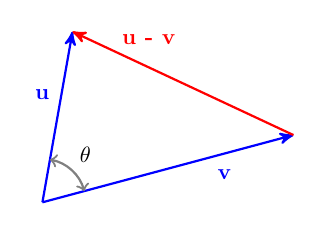
\begin{tikzpicture} [scale =1.1]

\coordinate (O) at (0,0);
\coordinate (u) at (80:2);
\coordinate (v) at (15:3);
\coordinate (d) at ($ (u) - (v) $);

\draw[blue, thick, ->,>=stealth'] (O) --(u) node[left, midway, yshift=5, yshift=3, scale=.8, text=blue]{\textbf{u}};
\draw[blue, thick, ->,>=stealth'] (O) --++(v) node[right, midway, xshift=15, yshift=-2, scale=.8, text=blue]{\textbf{v}};
\draw[red, thick, ->,>=stealth'] (v) --++(d) node[right, xshift=15, yshift=-3, scale=.8, text=red]{\textbf{u - v}};

\draw[gray,thick,<->] (15:.5) arc (15:80:.5) node[above right, midway, text=black, scale=.8]{$\theta$};

\end{tikzpicture}
\newline


hp9-3-53

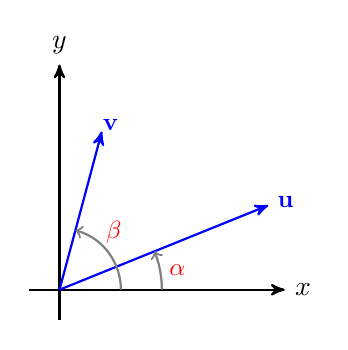
\begin{tikzpicture} [scale =1.3]
\draw[thick,->, >=stealth'] (-0.3,0) -- (2.2,0) node[anchor=west] {$x$};
\draw[thick,->, >=stealth'] (0,-0.3) -- (0,2.2) node[anchor=south] {$y$};
\def\a{22};
\def\b{75};
\coordinate (O) at (0,0);
\coordinate (u) at (\a:2.2);
\coordinate (v) at (\b:1.6);

\draw[blue, thick, ->,>=stealth'] (O) --(u) node[above right, yshift=-4, scale=.9, text=blue]{\textbf{u}};
\draw[blue, thick, ->,>=stealth'] (O) --++(v) node[above right, xshift=-3, yshift=-3, scale=.9, text=blue]{\textbf{v}};

\draw[gray,thick,->] (0:1) arc (0:\a:1) node[right, midway, text=red, scale=.9]{$\alpha$};
\draw[gray,thick,->] (0:0.6) arc (0:\b:.6) node[above, midway, xshift=2, text=red, scale=.9]{$\beta$};

\end{tikzpicture}
\newline

\section{Review}



hp9-rev-1ans.png

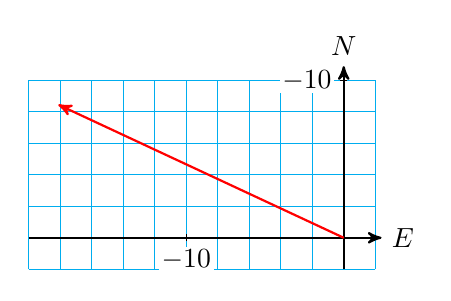
\begin{tikzpicture} [scale =.2]
\draw[cyan] (-20,-2) grid[step=2] (2,10);
\draw[thick,->, >=stealth'] (-20,0) -- (2.4,0) node[anchor=west] {$E$};
\draw[thick,->, >=stealth'] (0,-2) -- (0,10.9) node[anchor=south] {$N$};
\foreach \x in {10} {
    \draw (-\x,6pt) -- (-\x,-6pt) node[anchor=north, fill=white, inner sep=1, yshift=-2] {$-\x$};
    \draw (6pt,\x ) -- (-6pt,\x ) node[anchor=east, fill=white, inner sep=1, xshift=-2] {$-\x$};}
\coordinate (O) at (0,0);
\coordinate (v) at (155:20);

\draw[red, thick, ->,>=stealth'] (O) --(v) ;

\end{tikzpicture}
\newline



hp9-rev-3ans.png

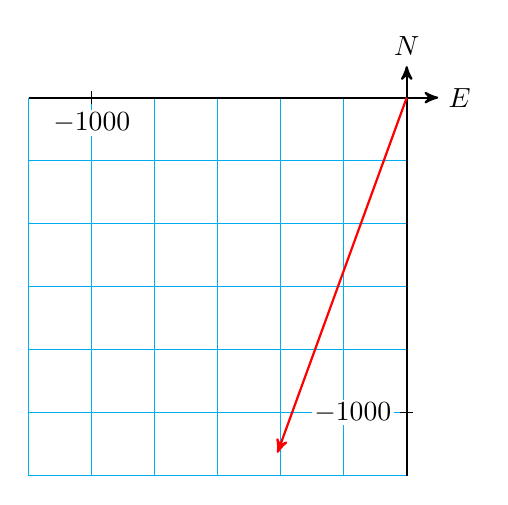
\begin{tikzpicture} [scale =.4]
\draw[cyan] (-12,-12) grid[step=2] (0,0);
\draw[thick,->, >=stealth'] (-12,0) -- (1.,0) node[anchor=west] {$E$};
\draw[thick,->, >=stealth'] (0,-12) -- (0,1.) node[anchor=south] {$N$};
\foreach \x in {10} {
    \draw (-\x,6pt) -- (-\x,-6pt) node[anchor=north, fill=white, inner sep=1, yshift=-2] {$-1000$};
    \draw (6pt,-\x ) -- (-6pt,-\x ) node[anchor=east, fill=white, inner sep=1, xshift=-2] {$-1000$};}
\coordinate (O) at (0,0);
\coordinate (v) at (250:12);

\draw[red, thick, ->,>=stealth'] (O) --(v) ;

\end{tikzpicture}
\newline



hp9-rev-9ans

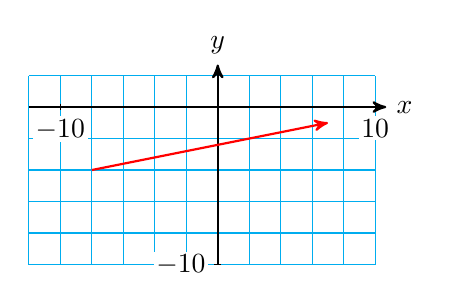
\begin{tikzpicture} [scale =.2]
\draw[cyan] (-12,-10) grid[step=2] (10,2);
\draw[thick,->, >=stealth'] (-12,0) -- (10.7,0) node[anchor=west] {$x$};
\draw[thick,->, >=stealth'] (0,-10) -- (0,2.7) node[anchor=south] {$y$};
\foreach \x in {10} {
    \draw (\x,6pt) -- (\x,-6pt) node[anchor=north, fill=white, inner sep=1, yshift=-2] {$\x$};
    \draw (-\x,6pt) -- (-\x,-6pt) node[anchor=north, fill=white, inner sep=1, yshift=-2] {$-\x$};
    \draw (6pt,-\x ) -- (-6pt,-\x ) node[anchor=east, fill=white, inner sep=1, xshift=-2] {$-\x$};}
\coordinate (O) at (-8,-4);
\coordinate (v) at (7,-1);

\draw[red, thick, ->,>=stealth'] (O) --(v) ;

\end{tikzpicture}
\newline



hp9-rev-11ans

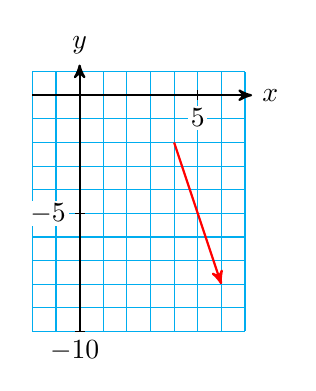
\begin{tikzpicture} [scale =.3]
\draw[cyan] (-2,-10) grid (7,1);
\draw[thick,->, >=stealth'] (-2,0) -- (7.3,0) node[anchor=west] {$x$};
\draw[thick,->, >=stealth'] (0,-10) -- (0,1.3) node[anchor=south] {$y$};
\foreach \x in {5} {
    \draw (\x,6pt) -- (\x,-6pt) node[anchor=north, fill=white, inner sep=1, yshift=-2] {$\x$};
    \draw (6pt,-\x ) -- (-6pt,-\x ) node[anchor=east, fill=white, inner sep=1, xshift=-2] {$-\x$};}
    \draw (6pt,-10) -- (-6pt,-10) node[anchor=north, fill=white, inner sep=1, yshift=-2] {$-10$};
\coordinate (O) at (4,-2);
\coordinate (v) at (6,-8);

\draw[red, thick, ->,>=stealth'] (O) --(v) ;

\end{tikzpicture}
\newline



hp9-rev-13ans

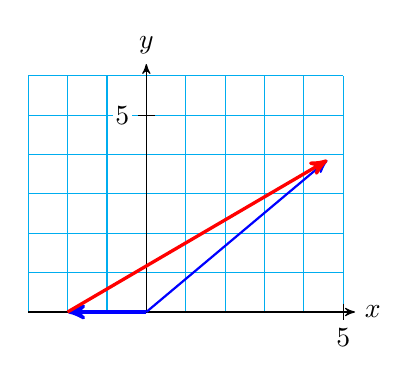
\begin{tikzpicture} [scale =.5]
\draw[cyan] (-3,0) grid (5,6);
\draw[->, >=stealth'] (-3,0) -- (5.3,0) node[anchor=west] {$x$};
\draw[->, >=stealth'] (0,0) -- (0,6.3) node[anchor=south] {$y$};
\foreach \x in {5} {
    \draw (\x,6pt) -- (\x,-6pt) node[anchor=north, fill=white, inner sep=1, yshift=-2] {$\x$};
    \draw (6pt,\x ) -- (-6pt,\x ) node[anchor=east, fill=white, inner sep=1, xshift=-2] {$\x$};}
\coordinate (O) at (0,0);
\coordinate (u) at (-2,0);
\coordinate (v) at (40:6);

\draw[blue, very thick, ->,>=stealth'] (O) --(u) ;
\draw[blue, thick, ->,>=stealth'] (O) --(v) ;
\draw[red, very thick, ->,>=stealth'] (u) --(v) ;

\end{tikzpicture}
\newline



hp9-rev-15ans

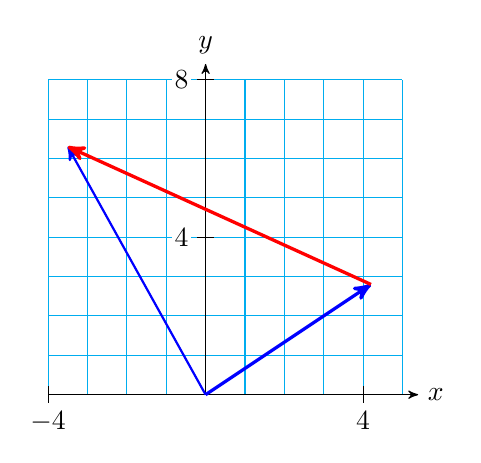
\begin{tikzpicture} [scale =.5]
\draw[cyan] (-4,0) grid (5,8);
\draw[->, >=stealth'] (-4,0) -- (5.4,0) node[anchor=west] {$x$};
\draw[->, >=stealth'] (0,0) -- (0,8.4) node[anchor=south] {$y$};
\foreach \x in {4,-4} {
    \draw (\x,6pt) -- (\x,-6pt) node[anchor=north, fill=white, inner sep=1, yshift=-2] {$\x$};}
\foreach \x in {4,8} {
    \draw (6pt,\x ) -- (-6pt,\x ) node[anchor=east, fill=white, inner sep=1, xshift=-2] {$\x$};}
\coordinate (O) at (0,0);
\coordinate (u) at (4.2,2.8);
\coordinate (v) at (-3.5,6.3);

\draw[blue, very thick, ->,>=stealth'] (O) --(u) ;
\draw[blue, thick, ->,>=stealth'] (O) --(v) ;
\draw[red, very thick, ->,>=stealth'] (u) --(v) ;

\end{tikzpicture}
\newline




hp9-rev-17

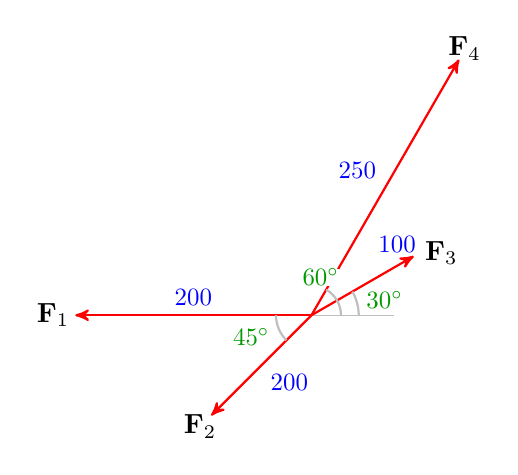
\begin{tikzpicture} [scale =.015]
\coordinate (O) at (0,0);
\coordinate (F1) at (180:200);
\coordinate (F2) at (225:120);
\coordinate (F3) at (30:100);
\coordinate (F4) at (60:250);

\node[xshift=-8] at (F1) {$\textbf{F}_1$};
\node[xshift=-4, yshift=-4] at (F2) {$\textbf{F}_2$};
\node[xshift=10, yshift=1] at (F3) {$\textbf{F}_3$};
\node[xshift=2, yshift=4] at (F4) {$\textbf{F}_4$};

\draw[lightgray] (O)--(70,0);
\draw[red, thick, ->,>=stealth'](O) --(F1) node[above, midway, text=blue, scale=.9]{200} ;
\draw[red, thick, ->,>=stealth'] (O) --(F2) node[below right, midway, text=blue, scale=.9]{200};
\draw[red, thick, ->,>=stealth'] (O) --(F3) node[above, xshift=-6, yshift=-2, text=blue, scale=.9]{100};
\draw[red, thick, ->,>=stealth'] (O) --(F4) node[above left, midway, text=blue, scale=.9]{250};

\draw[lightgray,thick] (180:30) arc(180:225:30) node[left, midway, yshift=-3, text=green!60!black, scale=.9] {$45\degree$};
\draw[lightgray,thick] (0:40) arc(0:30:40) node[right, midway, yshift=1, text=green!60!black, scale=.9] {$30\degree$};
\draw[lightgray,thick] (0:25) arc(0:60:25) node[above, xshift=-2, yshift=1, text=green!60!black, scale=.9, fill=white, inner sep=0] {$60\degree$};

\end{tikzpicture}
\newline




hp9-rev-18

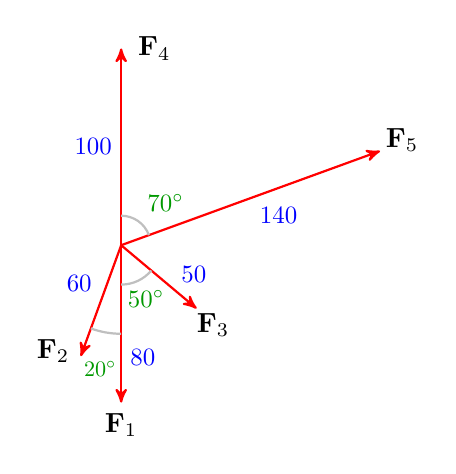
\begin{tikzpicture} [scale =.025]
\coordinate (O) at (0,0);
\coordinate (F1) at (270:80);
\coordinate (F2) at (250:60);
\coordinate (F3) at (-40:50);
\coordinate (F4) at (90:100);
\coordinate (F5) at (20:140);

\node[yshift=-8] at (F1) {$\textbf{F}_1$};
\node[xshift=-10, yshift=2] at (F2) {$\textbf{F}_2$};
\node[xshift=6, yshift=-6] at (F3) {$\textbf{F}_3$};
\node[xshift=12] at (F4) {$\textbf{F}_4$};
\node[xshift=8, yshift=4] at (F5) {$\textbf{F}_5$};

\draw[red, thick, ->,>=stealth'](O) --(F1) node[right, midway, yshift=-12, text=blue, scale=.9]{80} ;
\draw[red, thick, ->,>=stealth'] (O) --(F2) node[above left, midway, text=blue, scale=.9]{60};
\draw[red, thick, ->,>=stealth'] (O) --(F3) node[above, xshift=-1, yshift=6, text=blue, scale=.9]{50};
\draw[red, thick, ->,>=stealth'] (O) --(F4) node[left, midway, text=blue, scale=.9]{100};
\draw[red, thick, ->,>=stealth'] (O) --(F5) node[below right, midway, text=blue, scale=.9]{140};

\draw[lightgray,thick] (90:15) arc(90:20:15) node[above right, midway, text=green!60!black, scale=.9] {$70\degree$};
\draw[lightgray,thick] (-90:20) arc(-90:-40:20) node[below , midway, xshift=3, text=green!60!black, scale=.9] {$50\degree$};
\draw[lightgray,thick] (-90:45) arc(-90:-110:45) node[below, midway, xshift=-2, yshift=-10, text=green!60!black, scale=.8, fill=white, inner sep=0] {$20\degree$};

\end{tikzpicture}
\newline



\end{document}
